% ============================================================
% Informe TEST2 — demodulación AM/OOK con transformada de Hilbert,
% filtros FIR/IIR y filtrado espacial de imágenes.
%
% Mismo formato IEEEtran (conference) que WORK/REPORT/main.tex.
% Para compilar (Overleaf): pdflatex main.tex, dos pasadas.
% Las figuras están en figuras/ con prefijo por punto (punto1_, punto2_,
% punto3_).
% ============================================================

\documentclass[conference]{IEEEtran}

\usepackage[utf8]{inputenc}
\usepackage[T1]{fontenc}
\usepackage[spanish]{babel}

\usepackage{amsmath}
\usepackage{amssymb}

\usepackage{graphicx}
\usepackage{float}
\usepackage{booktabs}
\usepackage{array}

\usepackage{cite}
\usepackage{url}

\usepackage{xcolor}

\graphicspath{{figuras/}}

\title{
Demodulación de señales AM y OOK mediante la transformada de Hilbert,
filtros FIR/IIR y filtrado espacial de imágenes: informe TEST2
}

\author{
\IEEEauthorblockN{1\textsuperscript{st} Daniel García Araque}
\IEEEauthorblockA{
\textit{Programa de Ingeniería Mecatrónica}\\
\textit{Universidad Militar Nueva Granada}\\
Bogotá, Colombia\\
Cód. 7004185\\
est.daniel.garciaa@unimilitar.edu.co
}
\and
\IEEEauthorblockN{2\textsuperscript{nd} Karol Tatiana Fernández Neme}
\IEEEauthorblockA{
\textit{Programa de Ingeniería Mecatrónica}\\
\textit{Universidad Militar Nueva Granada}\\
Bogotá, Colombia\\
Cód. 7004191\\
est.karol.fernandez@unimilitar.edu.co
}
\and
\IEEEauthorblockN{3\textsuperscript{rd} Santiago Rubiano Garzón}
\IEEEauthorblockA{
\textit{Programa de Ingeniería Mecatrónica}\\
\textit{Universidad Militar Nueva Granada}\\
Bogotá, Colombia\\
Cód. 7004197\\
est.santiago.rigia@unimilitar.edu.co
}
}

\begin{document}

\maketitle

% RESUMEN

\begin{abstract}

Este informe presenta la solución de la evaluación TEST2, compuesta por
tres puntos. En el primero se analiza una señal de modulación de amplitud
(AM) almacenada en un archivo CSV: a partir de su espectro se midieron una
portadora de 20~kHz y un tono transmitido de 3~kHz (con bandas laterales
en 17 y 23~kHz), y se recuperó la envolvente mediante la magnitud de la
transformada de Hilbert seguida de filtros FIR e IIR pasa-bajas. Se
explica por qué un filtro centrado en la frecuencia del mensaje aplicado
directamente sobre la señal modulada no recupera la senoidal. En el
segundo punto se decodifica un mensaje transmitido por modulación de
encendido y apagado (OOK) a 1~kbit/s sobre una portadora de 10~kHz: la
envolvente de Hilbert se suaviza, se promedia por bit y se umbraliza,
obteniendo 144 bits que forman 18 bytes ASCII y la frase
``El Rey Leon (1994)''. En el tercer punto se ejecuta un código de filtrado
espacial con núcleos de $5\times5$ sobre una fotografía real, se justifica
que la convolución 2D es un filtro y se estudia el efecto de un núcleo
cuadrado de suma cero. Todos los valores y figuras provienen de la
ejecución real del código sobre los archivos entregados.

\end{abstract}

\begin{IEEEkeywords}

Modulación AM, modulación OOK, transformada de Hilbert, filtros FIR,
filtros IIR, decodificación ASCII, convolución 2D, filtrado espacial.

\end{IEEEkeywords}

% I. INTRODUCCIÓN

\section{Introducción}

La evaluación TEST2 propone tres ejercicios sobre archivos de datos
entregados: dos señales moduladas en formato CSV (columnas tiempo y
amplitud) y un código de filtrado de imágenes. Los archivos de las
señales siguen la convención \texttt{XX\_k\_modulated\_signal\_f\_fs\_T.csv},
donde $f$ es la frecuencia de la portadora en kHz, $f_s$ la frecuencia de
muestreo en kHz y $T$ la duración de la señal (punto 1) o el periodo de
bit (punto 2) en ms. Para este grupo se asignó el conjunto 01: la señal
del punto 1 tiene $f=20$~kHz, $f_s=200$~kHz y $T=40$~ms, y la del punto 2
tiene $f=10$~kHz, $f_s=100$~kHz y periodo de bit de 1~ms.

Los parámetros del nombre de archivo no se asumieron: se verificaron
contra las marcas de tiempo y el espectro de los propios datos. Cada punto
se implementó como un paquete Python independiente con pruebas
automatizadas, y este documento reúne los resultados obtenidos al ejecutar
ese código, junto con las explicaciones solicitadas. El código fuente
completo está disponible en
\url{https://github.com/DanielAraqueStudios/Signals-frecuency}, bajo
\texttt{THEORY/FIRST\_ROUND/TEST2/}.

La Sección~\ref{sec:resultados} desarrolla los tres puntos y la
Sección~\ref{sec:conclusiones} resume las observaciones principales.


\section{Resultados por punto}
\label{sec:resultados}

% ============================================================
% TEST2 Punto 1: AM, transformada de Hilbert y filtros FIR/IIR
% ============================================================

\subsection{Punto 1: Modulación AM, transformada de Hilbert y filtros FIR/IIR}

Este punto analiza la señal \texttt{01\_1\_modulated\_signal\_20.0\_200.0\_40.0.csv}: se revisa la modulación AM, se miden sobre los datos la portadora y el mensaje, se extrae la envolvente con la transformada de Hilbert filtrada con FIR e IIR, y se explica por qué un filtro centrado en la frecuencia del mensaje aplicado a la señal cruda no recupera el seno.

\subsubsection{(a) Revisión de la modulación AM}

En AM una señal mensaje de baja frecuencia $m(t)$ modula la amplitud de una portadora senoidal de alta frecuencia:
\begin{equation}
x(t) = \left[A_c + m(t)\right]\cos(2\pi f_c t).
\label{eq:t2p1_am}
\end{equation}
En frecuencia, el espectro de $m(t)$ se desplaza a $\pm f_c$: $x(t)$ tiene la portadora en $f_c$ y dos bandas laterales en $f_c \pm f_{msg}$, pero ninguna componente aislada en $f_{msg}$. Para recuperar $m(t)$ se usa detección de envolvente: la señal analítica $x_a(t) = x(t) + j\,\mathcal{H}\{x(t)\}$ tiene magnitud $|x_a(t)|$ que sigue a $A_c + m(t)$ mientras $f_c \gg$ el ancho de banda de $m(t)$, condición que aquí se cumple (portadora 20 kHz frente a mensaje de unos 3 kHz).

\subsubsection{(b) Frecuencias de portadora y mensaje}

Los valores se midieron directamente de los datos, no del nombre del archivo. La frecuencia de muestreo, $f_s = 1/\overline{\Delta t} = 200000{,}0$ Hz, y la duración, 39,995 ms (8000 muestras), coinciden con los valores nominales. El pico dominante de la FFT de la señal cruda está en \textbf{20000,0 Hz} (portadora), con bandas laterales simétricas en 17000 Hz y 23000 Hz, lo que confirma la estructura AM (Fig.~\ref{fig:t2p1_raw}). De las bandas laterales, $f_{msg} = 20000 - 17000 = $ \textbf{3000 Hz}, confirmado de forma independiente por la FFT de la magnitud de Hilbert, cuyo pico dominante fuera de DC está en 3000,0 Hz (Fig.~\ref{fig:t2p1_env}).

\begin{figure}[!t]
\centering
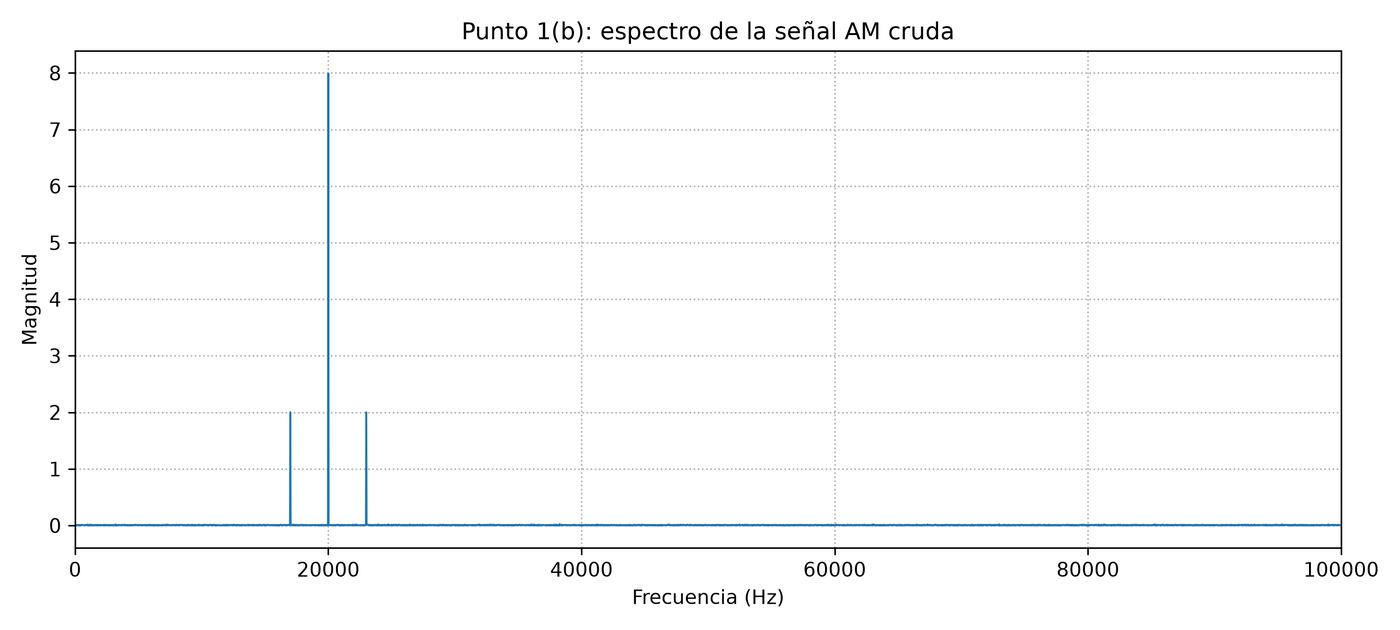
\includegraphics[width=\columnwidth]{punto1_p1_b_spectrum_raw.png}
\caption{Espectro de la señal AM cruda: portadora en 20 kHz y bandas laterales en 17 y 23 kHz.}
\label{fig:t2p1_raw}
\end{figure}

\begin{figure}[!t]
\centering
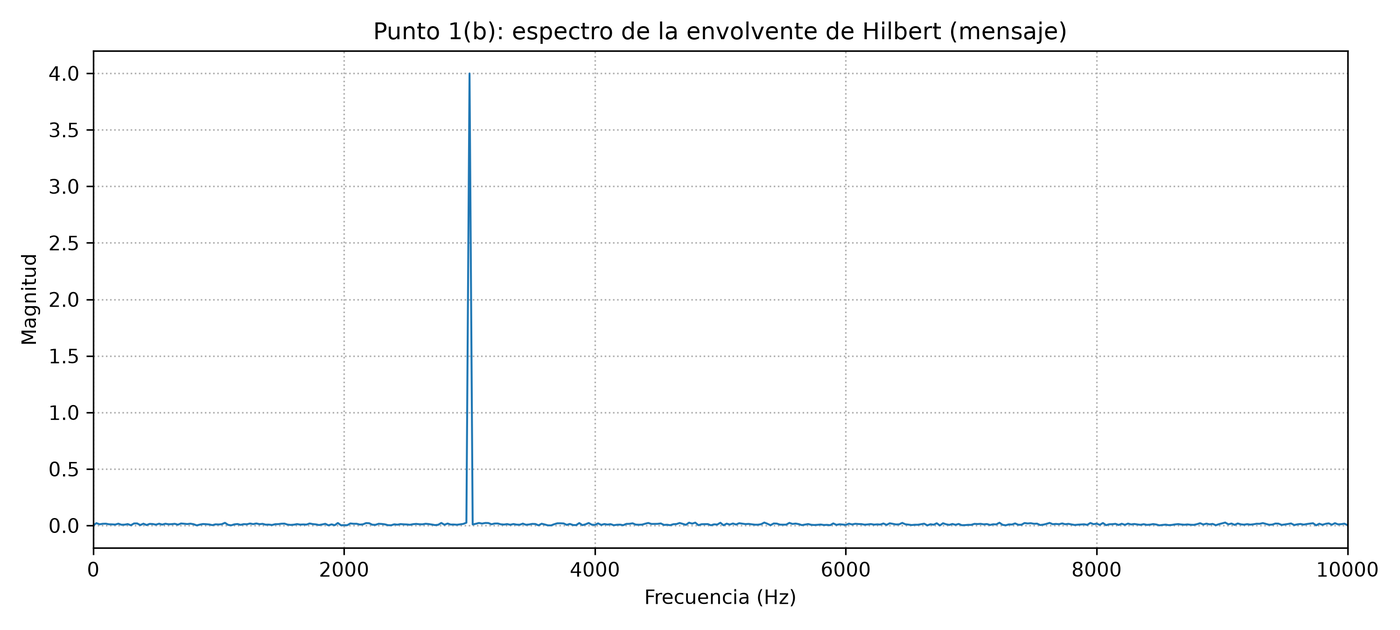
\includegraphics[width=\columnwidth]{punto1_p1_b_spectrum_envelope.png}
\caption{Espectro de la envolvente de Hilbert: el pico dominante (fuera de DC) está en 3 kHz.}
\label{fig:t2p1_env}
\end{figure}

\subsubsection{(c) Envolvente de Hilbert con filtro FIR}

Se calculó $|x_a(t)|$ con \texttt{scipy.signal.hilbert} y se filtró con un pasabajas FIR (\texttt{firwin}, fase cero con \texttt{filtfilt}) de corte 5000 Hz: por encima de los 3000 Hz del mensaje para no distorsionarlo y muy por debajo de los 20000 Hz de la portadora residual (Fig.~\ref{fig:t2p1_fir}).

\begin{figure}[!t]
\centering
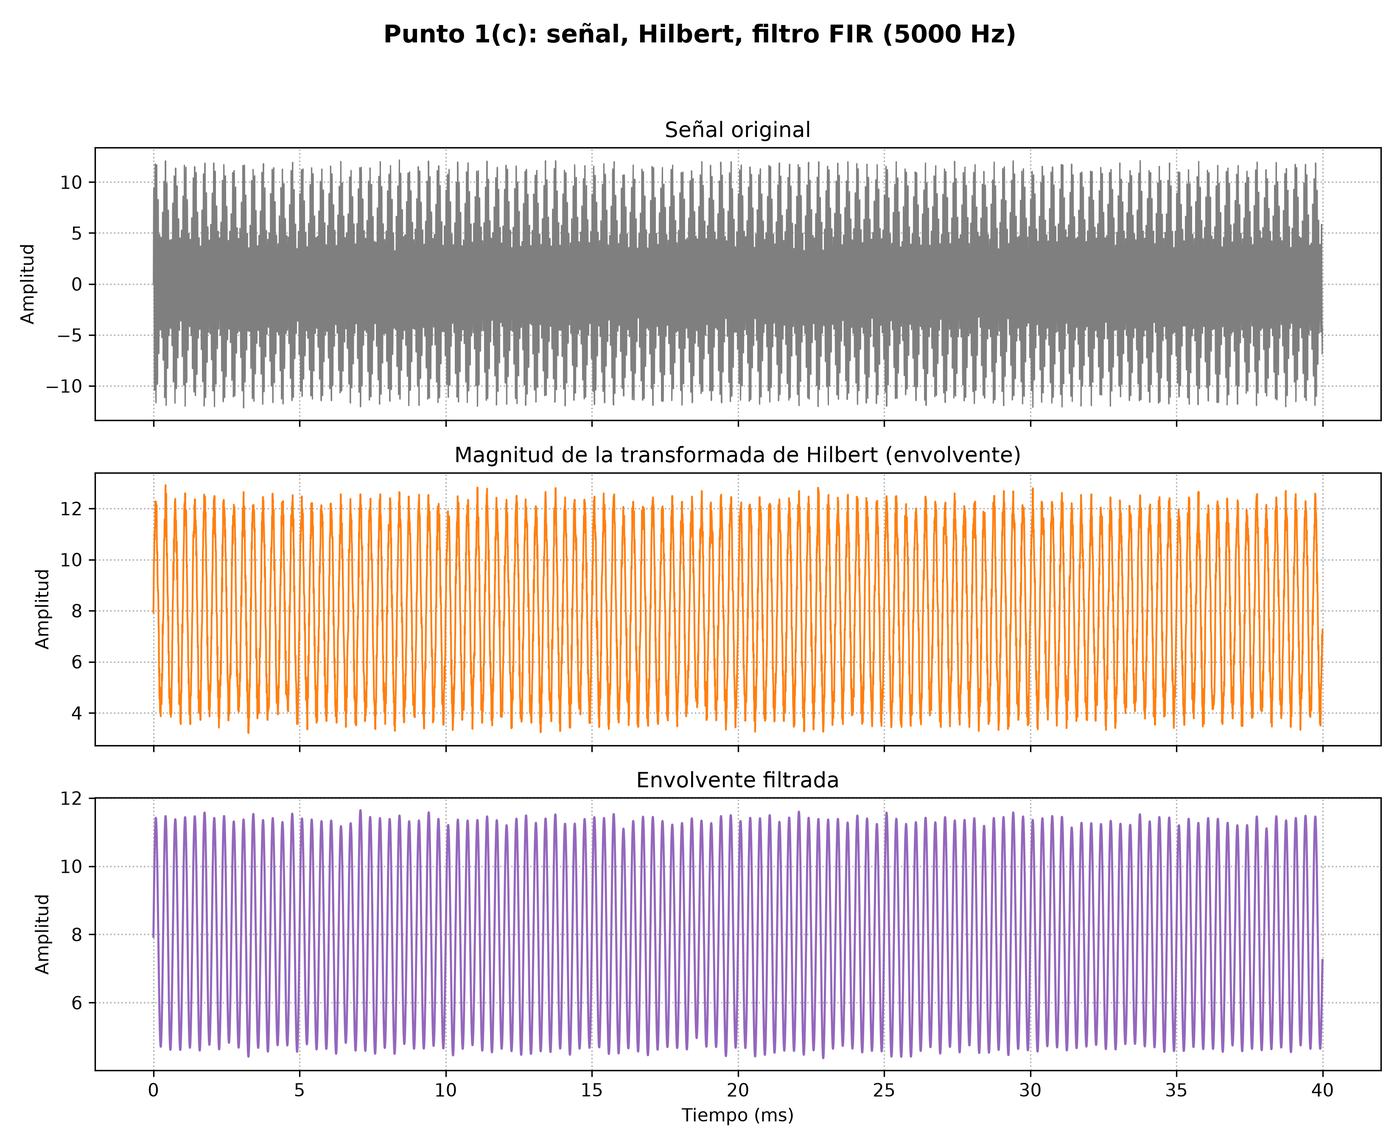
\includegraphics[width=\columnwidth]{punto1_p1_c_hilbert_fir.png}
\caption{Magnitud de Hilbert de la señal AM filtrada con un pasabajas FIR (corte 5 kHz).}
\label{fig:t2p1_fir}
\end{figure}

\subsubsection{(d) Envolvente de Hilbert con filtro IIR}

El mismo procedimiento con un pasabajas IIR Butterworth (\texttt{butter}, \texttt{filtfilt}), también con corte en 5000 Hz (Fig.~\ref{fig:t2p1_iir}).

\begin{figure}[!t]
\centering
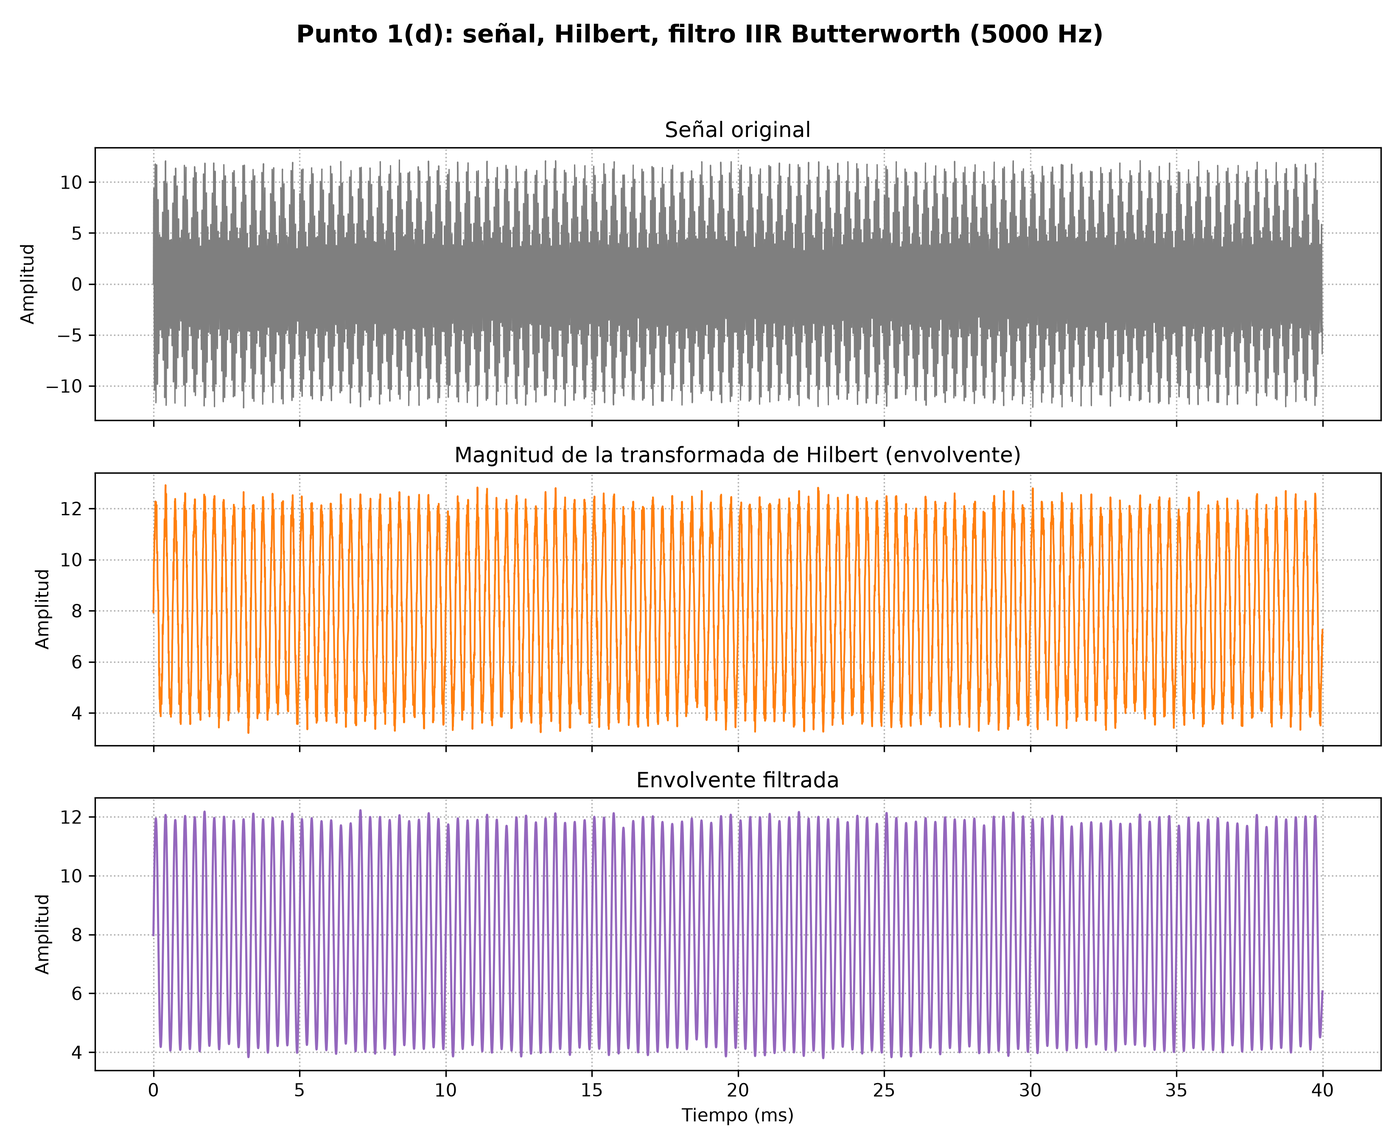
\includegraphics[width=\columnwidth]{punto1_p1_d_hilbert_iir.png}
\caption{Magnitud de Hilbert de la señal AM filtrada con un pasabajas IIR Butterworth (corte 5 kHz).}
\label{fig:t2p1_iir}
\end{figure}

\subsubsection{(e) Filtrado en $f_{msg}$ sobre la señal cruda}

Se diseñaron un pasabanda FIR de orden 50 y uno IIR Butterworth de orden 4, ambos centrados en $f_{msg} = 3000$ Hz (banda de 2500 a 3500 Hz), y se aplicaron a la señal AM cruda. Como muestran la Fig.~\ref{fig:t2p1_raw} y el panel inferior de la Fig.~\ref{fig:t2p1_target}, el espectro de $x(t)$ no tiene energía en 3000 Hz: su contenido está en 20 kHz y en 17/23 kHz, como predice la ecuación~\eqref{eq:t2p1_am}. Por eso el filtro no aísla ninguna componente del mensaje y solo deja pasar ruido numérico y fuga espectral, con amplitud muy inferior a la de la portadora; ni la salida FIR ni la IIR se parece a un seno de 3 kHz. El mensaje solo se recupera demodulando primero (Hilbert) para trasladarlo a banda base y filtrando después, como en (c) y (d).

\begin{figure}[!t]
\centering
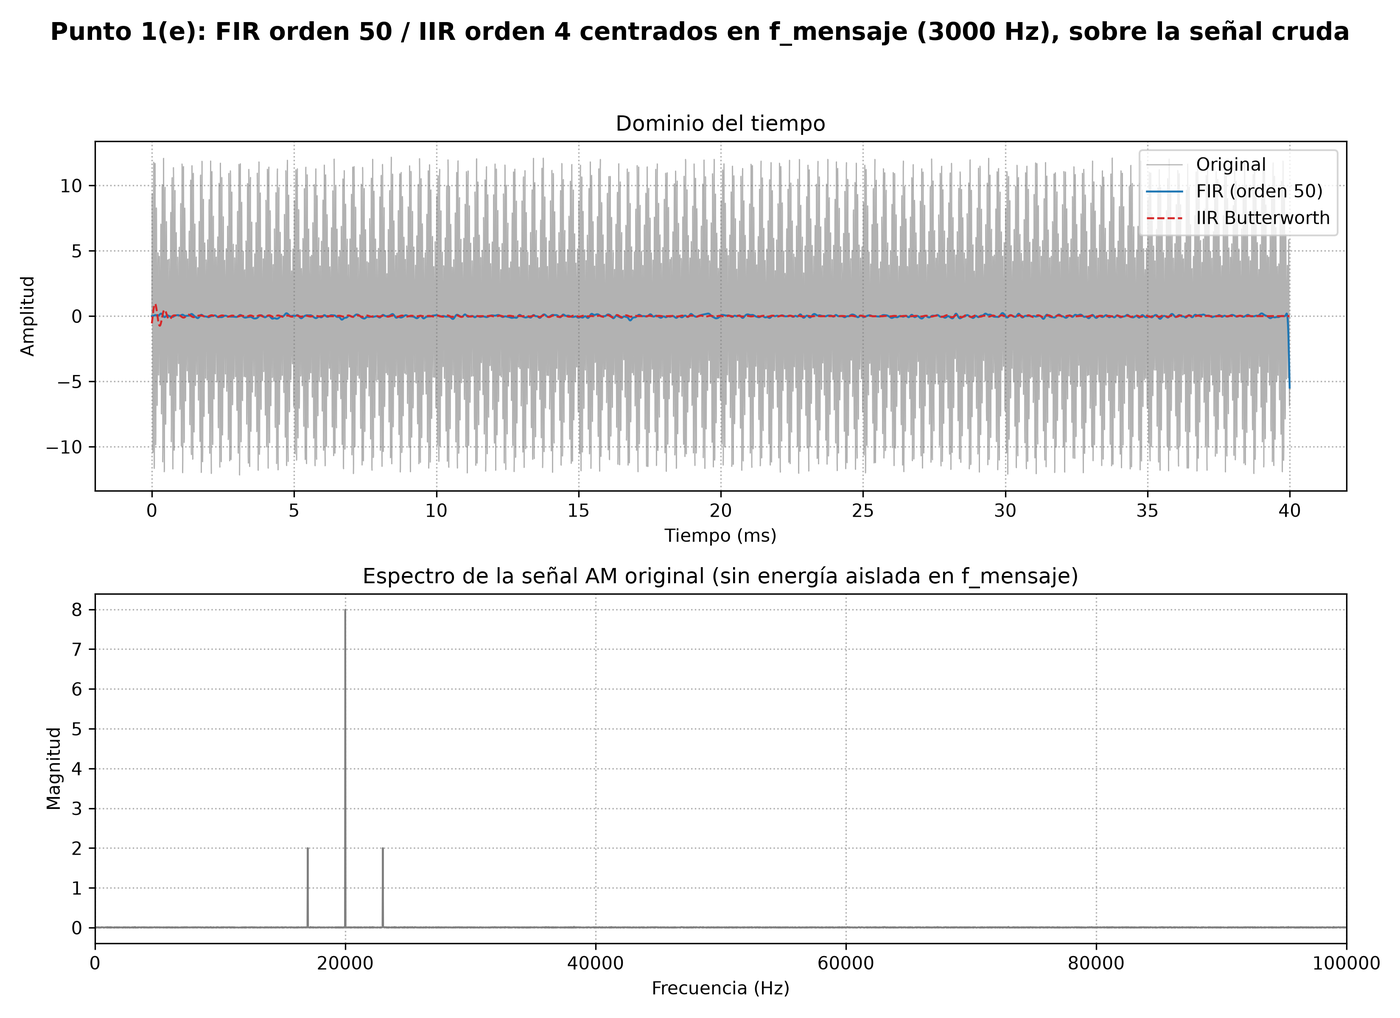
\includegraphics[width=\columnwidth]{punto1_p1_e_targeted_filter.png}
\caption{Pasabanda FIR (orden 50) e IIR (Butterworth, orden 4) en 3 kHz aplicados a la señal cruda: no recuperan un seno limpio.}
\label{fig:t2p1_target}
\end{figure}

\subsubsection{(f) Diferencias entre FIR e IIR}

\begin{itemize}
\item \textbf{Fase:} el FIR (\texttt{firwin}) es de fase lineal por diseño y el Butterworth de fase no lineal; al aplicar ambos con \texttt{filtfilt} la distorsión de fase neta se cancela, por lo que las diferencias visibles se deben a la forma del filtro.
\item \textbf{Transición:} para un mismo orden bajo, el Butterworth de orden 4 logra una banda de transición más angosta que el FIR de orden 50, a costa de fase no lineal y de posible inestabilidad numérica a órdenes altos.
\item \textbf{Rizado:} el FIR con ventana de Hamming tiene rizado moderado y predecible; el Butterworth es monótono en la banda de paso, pero cae más lentamente cerca del corte que un Chebyshev o elíptico del mismo orden.
\item \textbf{Estabilidad:} el FIR es siempre estable; el IIR depende de la ubicación de los polos, sin problema en el orden 4 usado aquí.
\end{itemize}

% ============================================================
% TEST2 Punto 2: Decodificacion de mensaje ASCII por OOK
% ============================================================

\subsection{Punto 2: Decodificación del mensaje ASCII transmitido por OOK}

Se analiza la señal \texttt{01\_2\_modulated\_signal\_10.0\_100.0\_1.0.csv}, una señal OOK (on/off keying) con portadora de 10 kHz. El archivo contiene 14\,400 muestras con $\Delta t = 10^{-5}$ s medido a partir de las marcas de tiempo reales, es decir $f_s = 100$ kHz y una duración de 0.14399 s. Con $T = 1$ ms por bit resultan 144 bits, o sea 18 bytes, compatibles con un mensaje ASCII de 18 caracteres.

\subsubsection{(a) Filtrado FIR/IIR a la frecuencia de bit}

Se diseñaron un filtro FIR pasabajas de orden 50 (\texttt{firwin}) y un Butterworth IIR de orden menor a 10 (\texttt{butter}), ambos con corte en la frecuencia de bit $1/T = 1$ kHz y aplicados en fase cero con \texttt{filtfilt} directamente sobre la señal cruda. Como muestra la Fig.~\ref{fig:punto2_t2a_spectrum}, la energía de la señal OOK, $\text{envolvente}(t)\sin(2\pi f_c t)$ con $f_c = 10$ kHz, se concentra alrededor de la portadora y no en 1 kHz, donde el espectro es prácticamente vacío. Por ello un pasabajas de 1 kHz solo elimina la portadora y deja una traza casi plana o ruidosa, sin la onda cuadrada de bits (Fig.~\ref{fig:punto2_t2a_filtered}). Para recuperar la envolvente es necesario demodular antes de filtrar.

\begin{figure}[!t]
\centering
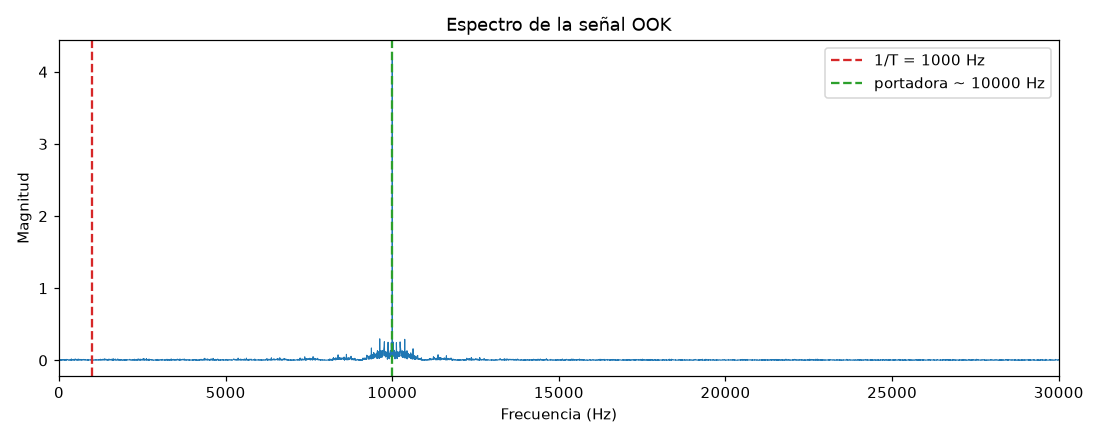
\includegraphics[width=\columnwidth]{punto2_t2a_spectrum.png}
\caption{Espectro FFT de la señal OOK: la energía se concentra cerca de la portadora de 10 kHz.}
\label{fig:punto2_t2a_spectrum}
\end{figure}

\begin{figure}[!t]
\centering
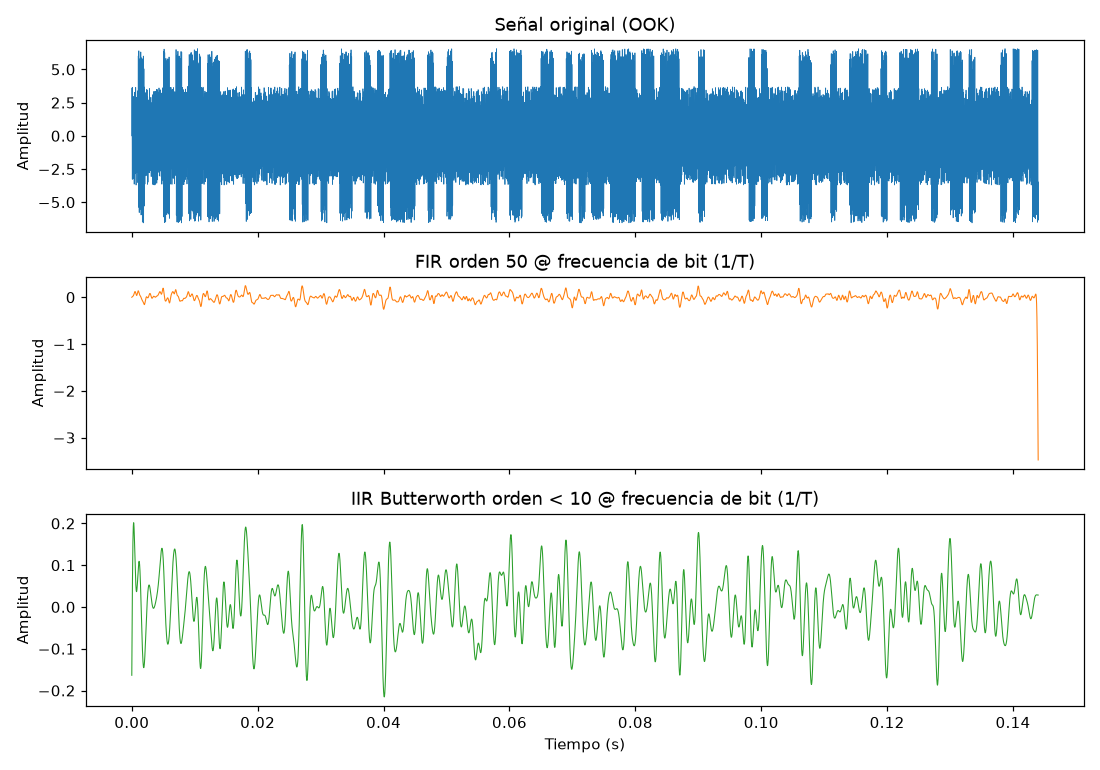
\includegraphics[width=\columnwidth]{punto2_t2a_filtered_bit_rate.png}
\caption{Salidas de los filtros FIR (orden 50) e IIR (Butterworth) con corte en 1 kHz sobre la señal cruda: no aparece el patrón cuadrado.}
\label{fig:punto2_t2a_filtered}
\end{figure}

\subsubsection{(b) Envolvente de Hilbert y reconstrucción de bits}

La magnitud de la señal analítica (\texttt{scipy.signal.hilbert}) entrega la envolvente on/off. Esta se suaviza con un pasabajas a $0.3/T$ para eliminar el rizado de portadora conservando las transiciones. Luego se promedia la envolvente en cada ventana de 1 ms y los 144 promedios se separan en dos grupos (alto/bajo) con un 2-means unidimensional; el umbral adaptativo es el punto medio entre los centroides convergidos, de modo que se autocalibra a los niveles reales de la señal. La Fig.~\ref{fig:punto2_t2b} muestra la señal cruda, la magnitud de Hilbert y la onda cuadrada reconstruida.

\begin{figure}[!t]
\centering
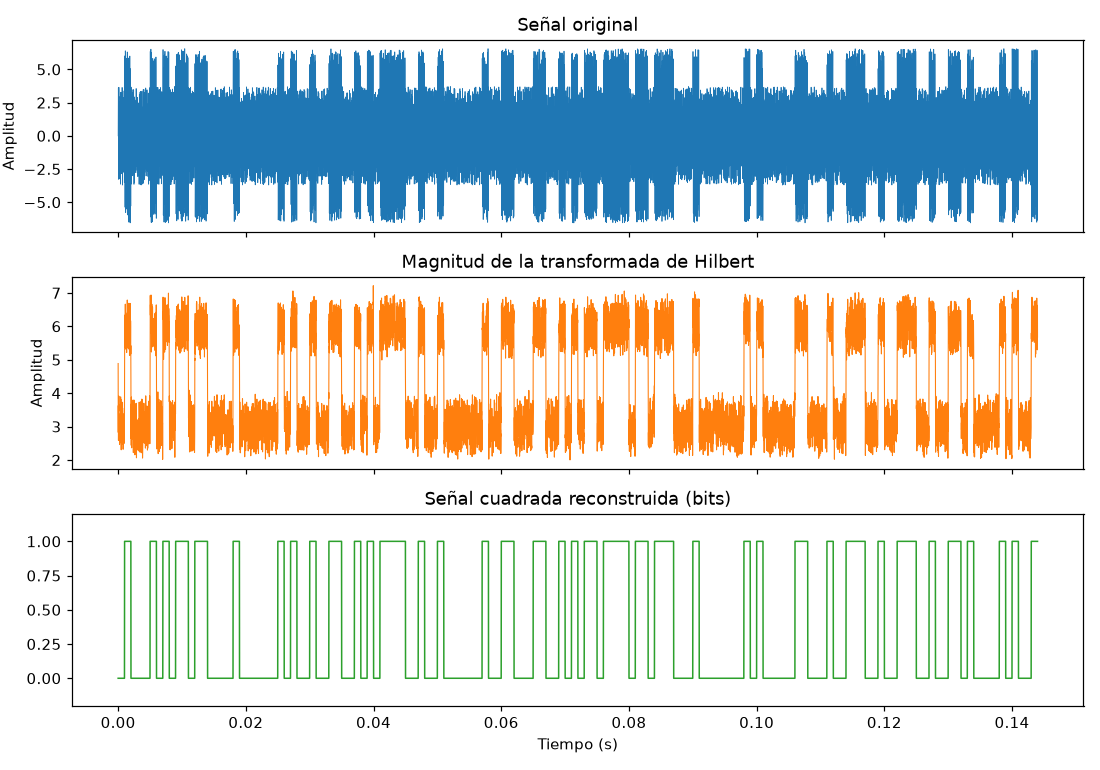
\includegraphics[width=\columnwidth]{punto2_t2b_hilbert_bits.png}
\caption{Señal cruda, magnitud de Hilbert y onda cuadrada reconstruida a partir de los bits detectados.}
\label{fig:punto2_t2b}
\end{figure}

\subsubsection{(c) Decodificación ASCII}

Los 144 bits recuperados se agrupan en 18 bytes de 8 bits. Se evaluaron los 16 candidatos posibles (8 desfases de bit $\times$ {MSB primero, LSB primero}) puntuando por cantidad de bytes ASCII imprimibles. La única combinación con 18/18 bytes imprimibles es desfase 0 con MSB primero; el resto obtuvo puntajes muy inferiores (Tabla~\ref{tab:punto2_decode}). El mensaje decodificado es

\begin{center}
\texttt{El Rey Leon (1994)}
\end{center}

\begin{table}[!t]
\centering
\caption{Búsqueda de desfase y orden de bits.}
\label{tab:punto2_decode}
\begin{tabular}{lcc}
\toprule
Configuración & Candidatos & Imprimibles \\
\midrule
Desfase 0, MSB primero & 1 & 18/18 \\
Otros desfases y LSB primero & 15 & muy inferior \\
\bottomrule
\end{tabular}
\end{table}

Para validar el pipeline (envolvente $\to$ suavizado $\to$ umbral por bit $\to$ ASCII) se construyó una señal OOK sintética con la cadena conocida \texttt{Hi DSP!}, y la prueba automática de ida y vuelta recupera exactamente esa cadena (desfase 0, MSB primero). Las 5 pruebas del laboratorio pasan.

% ============================================================
% PUNTO 3: Filtrado espacial de imágenes con núcleos 2D
% ============================================================

\subsection{Punto 3: Filtrado espacial de una imagen con núcleos 2D}

\subsubsection{Descripción del código}

El código adjunto (\texttt{cod01.py}) carga una imagen, la convierte a
escala de grises y le aplica convolución discreta 2D mediante
\texttt{cv2.filter2D} con núcleos fijos de $5\times5$: un núcleo
promediador (\texttt{kernel\_pasa\_bajas}, todos los coeficientes iguales
a $0.04$), dos núcleos con centro positivo fuerte y entorno negativo
(\texttt{kernel\_pasa\_altas00} y \texttt{kernel\_pasa\_altas02}) y una
cascada pasa-bajas seguida de pasa-altas denominada ``Filtro Pasa
Bandas''. Como el código original usa \texttt{cv2.imshow}, se adaptó a un
entorno sin ventana gráfica guardando cada resultado como imagen, sin
modificar los núcleos ni las llamadas a \texttt{filter2D}. Se empleó como
entrada una fotografía real de una tarjeta débito sobre una mesa de
madera (Fig.~\ref{fig:t2p3_orig}), que aporta bordes nítidos (logotipo,
chip, contorno de la tarjeta), regiones planas (el fondo amarillo) y
textura fina (la veta de la madera).

Las sumas de coeficientes, calculadas numéricamente y verificadas con
pruebas automáticas, son: \texttt{kernel\_pasa\_bajas} $=1.0$,
\texttt{kernel\_pasa\_altas00} $=1.0$, \texttt{kernel\_pasa\_altas02}
$=0.0$ y el núcleo nuevo del inciso (b) $=0.0$. Nótese que
\texttt{kernel\_pasa\_altas00}, pese a su nombre, no suma cero.

\begin{figure}[!t]
\centering
\begin{minipage}{0.48\columnwidth}
\centering
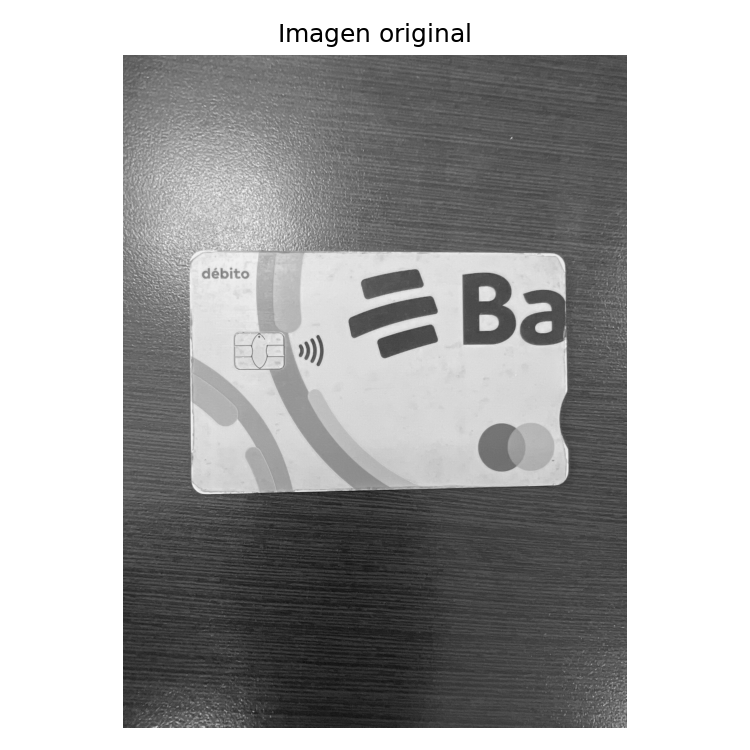
\includegraphics[width=\linewidth]{punto3_00_original.png}
\end{minipage}\hfill
\begin{minipage}{0.48\columnwidth}
\centering
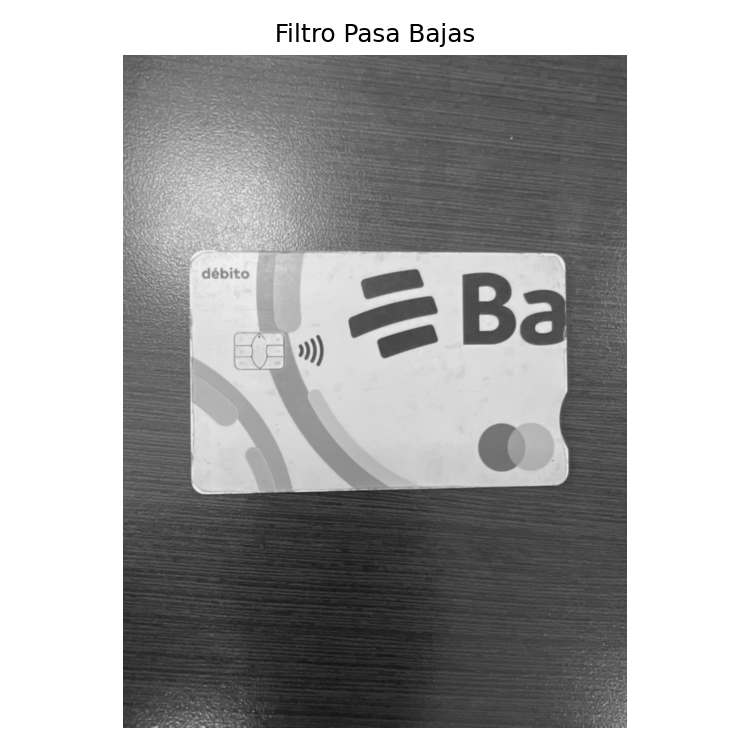
\includegraphics[width=\linewidth]{punto3_01_pasa_bajas.png}
\end{minipage}
\caption{Imagen de entrada en escala de grises (izquierda) y resultado del filtro pasa-bajas de $5\times5$ (derecha): la veta de la madera y los bordes se suavizan, pero el brillo medio se conserva.}
\label{fig:t2p3_orig}
\end{figure}

\begin{figure}[!t]
\centering
\begin{minipage}{0.48\columnwidth}
\centering
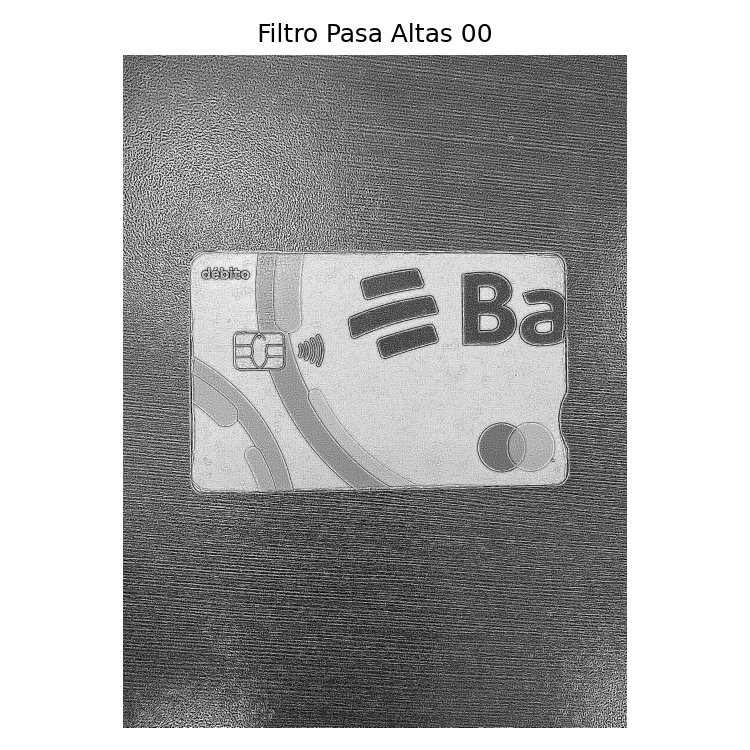
\includegraphics[width=\linewidth]{punto3_02_pasa_altas00.png}
\end{minipage}\hfill
\begin{minipage}{0.48\columnwidth}
\centering
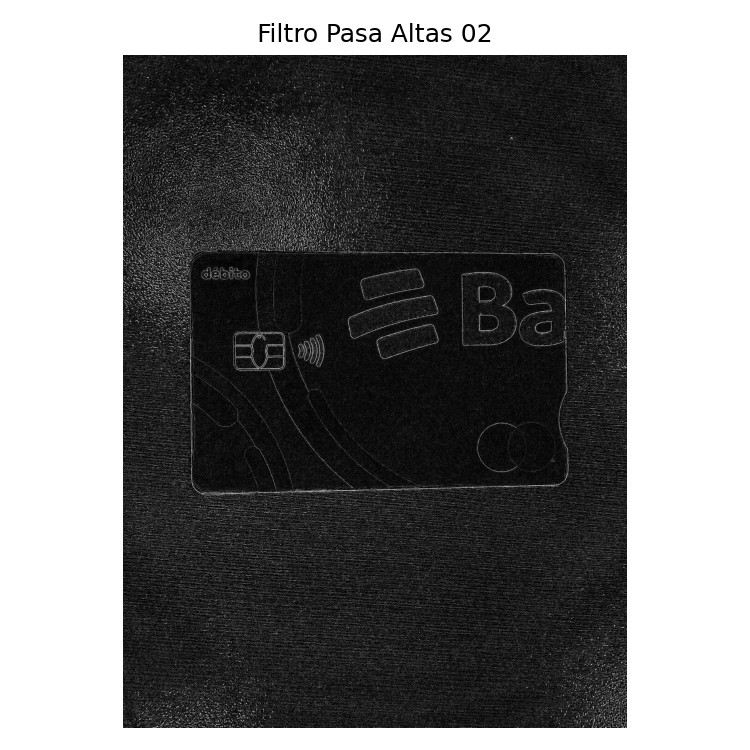
\includegraphics[width=\linewidth]{punto3_03_pasa_altas02.png}
\end{minipage}
\caption{Resultado de \texttt{kernel\_pasa\_altas00} (izquierda, suma $=1$) y \texttt{kernel\_pasa\_altas02} (derecha, suma $=0$).}
\label{fig:t2p3_altas}
\end{figure}

\begin{figure}[!t]
\centering
\begin{minipage}{0.48\columnwidth}
\centering
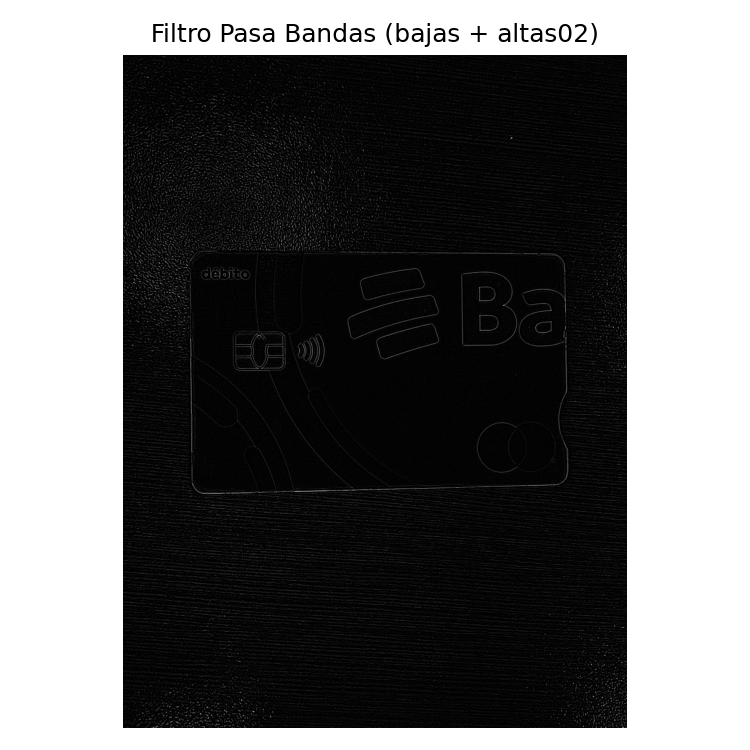
\includegraphics[width=\linewidth]{punto3_04_pasa_bandas.png}
\end{minipage}\hfill
\begin{minipage}{0.48\columnwidth}
\centering
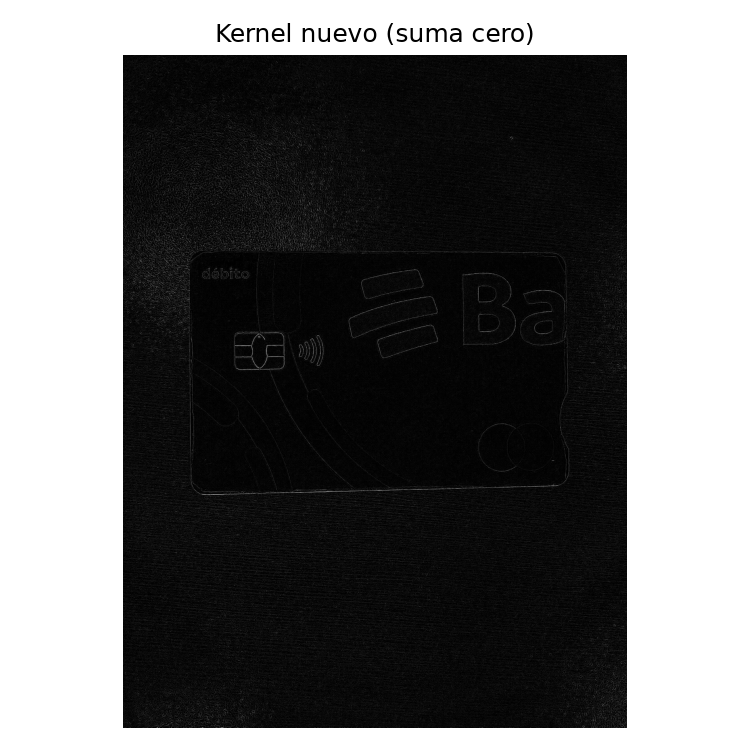
\includegraphics[width=\linewidth]{punto3_05_kernel_nuevo.png}
\end{minipage}
\caption{Cascada pasa-bajas más \texttt{kernel\_pasa\_altas02} (izquierda) y núcleo nuevo de suma cero, Laplaciano de $3\times3$ (derecha).}
\label{fig:t2p3_nuevo}
\end{figure}

\subsubsection{(a) ¿Se puede considerar un filtro?}

Sí. La convolución con un núcleo fijo es, por definición, un filtro lineal
e invariante al desplazamiento: la operación
$y[m,n]=\sum_i\sum_j h[i,j]\,x[m-i,n-j]$ es la misma convolución de un
filtro FIR unidimensional, aplicada sobre dos ejes. Cada núcleo es una
respuesta al impulso de soporte finito, equivalente al vector de
coeficientes de un FIR. El núcleo pasa-bajas (suma $1$, todos positivos)
es un promedio móvil bidimensional: atenúa las frecuencias espaciales
altas (bordes y textura fina) y conserva el brillo local, como se observa
en la Fig.~\ref{fig:t2p3_orig}. Los núcleos con centro positivo y entorno
negativo se comportan como un Laplaciano discreto: responden donde el
brillo cambia rápido (contorno de la tarjeta, letras, chip) y poco en
regiones uniformes. \texttt{kernel\_pasa\_altas02} (Fig.~\ref{fig:t2p3_altas},
derecha) deja el fondo amarillo casi negro y solo resalta los bordes,
mientras que \texttt{kernel\_pasa\_altas00} (izquierda) conserva la imagen
completa y añade realce de detalle, porque su suma es $1$ y por tanto aún
deja pasar la componente de continua. La cascada (Fig.~\ref{fig:t2p3_nuevo},
izquierda) actúa como un pasa-bandas: primero elimina el ruido de muy alta
frecuencia y luego extrae los bordes, produciendo líneas más limpias y
tenues que \texttt{kernel\_pasa\_altas02} solo.

\subsubsection{(b) Cambio de la matriz con suma cero}

Se definió un núcleo nuevo, cuadrado y de suma cero, el Laplaciano
discreto de $3\times3$:
\begin{equation}
h=\begin{bmatrix}1&1&1\\1&-8&1\\1&1&1\end{bmatrix},\qquad
\sum_{i,j}h[i,j]=0.
\end{equation}
Un núcleo de suma cero no tiene ganancia en continua: sobre una región
uniforme de $128$ niveles de gris la salida de \texttt{filter2D} es
exactamente $0$ en todo el interior (verificado con una prueba
automática), sin importar el brillo original, y sobre un borde abrupto la
respuesta es grande ($|y|>20$). El núcleo se convierte así en un detector
de bordes puro que descarta la información de brillo. Comparado sobre la
misma región plana, \texttt{kernel\_pasa\_altas00} (suma $1$) devuelve
$128$, mientras que \texttt{kernel\_pasa\_altas02} y el núcleo nuevo
(suma $0$) devuelven $0$. En la imagen real (Fig.~\ref{fig:t2p3_nuevo},
derecha) el fondo y el interior de la tarjeta quedan negros y solo
permanecen los contornos, más finos y tenues que con el núcleo de
$5\times5$ porque el soporte es menor. Al cambiar los valores del núcleo
manteniendo suma cero, las regiones planas siempre desaparecen; lo que
cambia es la intensidad y el patrón con que responden los bordes. Además,
como \texttt{filter2D} trabaja con salida \texttt{uint8}, las respuestas
negativas se saturan a $0$ y solo se visualiza la parte positiva de la
respuesta al borde.


% CONCLUSIONES

\section{Conclusiones}
\label{sec:conclusiones}

En los puntos 1 y 2 el resultado central es el mismo: en una señal
modulada, la información no está en el espectro a la frecuencia del
mensaje o de los bits, sino alrededor de la portadora. Por eso un filtro
FIR de orden 50 o un Butterworth de orden menor a 10 centrado en 3~kHz
(punto 1) o en 1~kHz (punto 2) y aplicado directamente sobre la señal
cruda no recupera la senoidal ni la onda cuadrada. Primero hay que
demodular, aquí con la magnitud de la transformada de Hilbert, y solo
después filtrar la envolvente.

Las frecuencias se midieron de los datos: portadora de 20~kHz y mensaje de
3~kHz en el punto 1, con bandas laterales en 17 y 23~kHz que confirman la
estructura AM. En el punto 2, la decodificación se validó con una prueba
de ida y vuelta sobre una señal OOK sintética de mensaje conocido y con la
búsqueda exhaustiva de alineación de byte y orden de bits, cuyo único
candidato con 18 de 18 caracteres imprimibles es
``El Rey Leon (1994)''.

En el punto 3, un núcleo cuya suma es cero elimina la componente de
continua, de modo que las regiones uniformes se anulan y solo responden
los bordes; el nombre de un núcleo no garantiza esta propiedad, como
muestra \texttt{kernel\_pasa\_altas00}, cuya suma real es $1$.

% REFERENCIAS

\begin{thebibliography}{00}

\bibitem{oppenheim}
A. V. Oppenheim, A. S. Willsky y S. H. Nawab,
\textit{Signals and Systems},
2nd ed., Prentice Hall, 1996.

\bibitem{oppenheimschafer}
A. V. Oppenheim y R. W. Schafer,
\textit{Discrete-Time Signal Processing},
3rd ed., Pearson, 2010.

\bibitem{lyons}
R. G. Lyons,
\textit{Understanding Digital Signal Processing},
3rd ed., Pearson, 2011.

\bibitem{gonzalez}
R. C. Gonzalez y R. E. Woods,
\textit{Digital Image Processing},
4th ed., Pearson, 2018.

\bibitem{numpy}
C. R. Harris et al.,
``Array programming with NumPy,''
\textit{Nature}, vol. 585, pp. 357--362, 2020.

\bibitem{scipy}
P. Virtanen et al.,
``SciPy 1.0: Fundamental Algorithms for Scientific Computing in Python,''
\textit{Nature Methods}, vol. 17, pp. 261--272, 2020.

\bibitem{opencv}
G. Bradski,
``The OpenCV Library,''
\textit{Dr. Dobb's Journal of Software Tools}, 2000.

\end{thebibliography}


\end{document}
